\chapter{Experiments and Testing}
\label{chapter:4}
%% NO PERSONAL FORMS us,we,I
%% quotes use like : ``text''
%% after point,doublepoints and commas there must be a BLANK SPACE

% **************************** Define Graphics Path **************************
\ifpdf
    \graphicspath{{Chapter3/Figs/Raster/}{Chapter3/Figs/PDF/}{Chapter3/Figs/}}
\else
    \graphicspath{{Chapter3/Figs/Vector/}{Chapter3/Figs/}}
\fi

This Chapter is a detailed description about the simulations and experiments of the Invariant Observer.
The first section introduce a survey about the test environment and their different configurations.
The second section shows something about the simulations and their conclusions.
The third section is a detailed description about the test cases and experiments,even something about the performance studies which where
discussed in the chapter before. \\



\section{Reasoning and Environment of Experiments}
This section should be considered as a description about the questions ``Which result do we gain from these experiments?'' and ``How are the experiments done?''. 

\subsection{Reasoning and Meaning}
The Invariant Observer will interact in an environment where at least soft real-time, but rather hard real-time conditions, should be fullfilled.
The first step, to show  correct behaviour of the algorithm and the resulting VHDL Implementation, are simulations. But it should be mentioned that no 
clear assertions can be made about correct timings. This question relies on the part of experiments. How the simulations and experiments were done, and which insights
they produced, will be discussed in the next subsection.
To present a first proof about correct principle of the Invariant Observer it was necessary to synthesize the VHDL Implementation to get a prototype.
A FPGA was the best solution, besides other possibilities like ASIC's or a Microcontroller. An ASIC (Application-specific integrated circuit) is the most performant solution, but
that solution is hardwired and any change of the design is very expensive. But it could be considered as the final product implementation.
A Microcontroller would never reach the performance of a FPGA and FPGA's are more cost effective and nearly performant like hardwired solutions. 
Any change of the design can be easily downloaded on a FPGA Board, so it seems logical to use FPGA's as protoyping platform.
One important aspect of the experiments was to show the timings of the design. 
for example to show the maximum performance on a FPGA board like the DE2-115, which was used for the expriments, as already mentioned.
But other FPGA's with stronger abilities could reach better performance goals. In \cite{RTFMBJ13} several FPGA models were used to show that aspect.      
A further aspect was to show the ability of handling any propositional formula $\phi$, which is composed of several possible input signals.
The evaluation of $\phi$ takes time, maybe several clock cycles. That circumstance was not exactly tested, but a different approach was
tried to show the same way. A more exact test could be done if this work will be continued.
The next subsection will explain the actual investigations of the experiments in great detail.  
\subsection{Build-up of Experiments}
At first some facts about the Invariant Observer will be repeated, to give a better understanding about the tests that were made.
The Invariant Observer consist of several Observer Stages. Every Observer Stage hast to wait, at least the time needed to evalaute a proposition $\phi$, until
th evaluation finished. To cover every clock cycle $e^n$, where a finished computation of a proposition $W(\phi)$ will be evaluated, we need least as many Observer Stages, as
the computation (m clock cycles) needs. To remind, the observer stages are not responsible for the computation of the propositions(like in \cite{RTFMBJ13} ),
but for the final evaluation of the status of the computation.
So it seems logical to create a signal $\phi$ which gives, at every clock cycle, a pseudo evaluation of an proposition $\phi$. 
After that it was easy to show the correct beahviour of the Invariant Observer. 
For example we have m=3 Observer (means theoretical that the evaluation needs 3 clock cycles), and want to show the invariance of signal $\phi$, actually the finished computation $W(\phi)$,
with $\tau = 10$. That 3 Observer Stages shows whether the $W(\phi)$ was invariant 10 clock cycles before and the current clock cycle.
The experiments have been exercised with a plain implementation of a signal $W(\phi)$ and with a more complex implementation of $W(\phi)$, which gives a stronger argument of the correct behaviour.
More about that in the simulation section and experiment section.
That two versions of simulating the input signal of the observer are justified with the fact, that the Quartus synthesis tool could create distinct implementations of the Observer Design, because it must
match the correct timing behaviours. This will be discussed in the experiment section       
The experiments consists of a plain Observer Stage with different configurations with the plain input and the complex input. The same with several Observer Stages.
The next section gives us an insight about the simulations.
%
%A) Reason for tests (behaviour,design improvements,faster design)
%\subsection{}
%B) Test Board , Analyzer ,Versions, Configurations? 
%PF2 -Sampling rate Logic Analyzer

%Top.vhd
%Signalgenerator.vhd

%
%% + SOMETHING ABOUT sIGNALGENERATOR



\section{Simulations}
To simulate the VHDL Design of the Observer Stages  the simulation tool \textbf{ModelSim (Version 10.1d)} from \textbf{MentorGraphics} was used.  
A testbench created for simulations in Modelsim gives a good overview about the intended behaviour of the implemented algorithm and it is usefull for debugging and error detection.
At the beginning, only one Observer Stage was simulated, because it demonstrates the simplest case. After error corrections and succesfull simulation of one Observer Stage, which behaves 
like an native Invariance Observer, simulations were proceed with more Observer Stages.\\
 
In Figure~\ref{fig:simulation:five} there is illustrated a simulation with m=5 Observer, where every observer stage monitors the yellow-colored input signal $\phi$ for Invariance $\tau=3$.
The most left column shows the names of the illustrated signals. For every Observer (OBS1 to OBS5), signals cycle, $count_p$ and their outputs (add1 to add5) are shown to overlook their
behaviour on input signal $phi\_s$ (=$\phi$). Signals cycle and $count_p$ are already descibed in Chapter~\ref{chapter:3}, so there is nothing additional.
Signals add1 to add5 are the outputs of the different Observer Stages, which are linked together in a binary add operation.
The result of that operation is illustrated as the red-colored signal $output_s$ which shows the final result of the Invariance Observer.\\
Signal $phi\_s$ is generated by a complex signalgenerator to get a nearly universal test signal. The green-colored signal at the top indicates the system clock which drives the signalgenerator
with his output $phi\_s$ and all the observer stages at the same time. But the signalgenerator is driven on the rising edge, the Oberver Stages on falling edge.
This fact is important to understand one further explanations of the simulation. 
The most important thing that is shown in that illustration is that the observer stages activate the final $output\_s$ exactly $tau + 1$  clock cycles after signal phi\_s still holds his active state.
This case is  indicated between the two big vertical lines. 
This shows that the Invariance Observer monitored an Invariance Situation of signal $phi\_s$, according to the behaviour described in Chapter~\ref{chapter:2}. 
The Invariance Situation continues three clock cycles until signal phi\_s goes into a non active state. \\
As mentioned, signal phi\_s changes his states on every rising edge, whereas a Observer Stage checks the state of signal phi\_s on every falling edge. 
This explains the delayed reaction of the Observer Stages on changes of the input signal. This handicap could be enhanced by driving the Observers clock a multiple faster.
The signalgenerator is designed to increase the invariance of his active state continuously, so it was reasonable to see how the final red-colored output works. 
To make it clear, signal phi\_s which is created by the signalgenerator only delivers a pseudo input for the Observer Stages which can be understood like as, at every clock cycle, a computation of
$W(\phi)$ is finished and the result of that computation is illustrated as true (active state) or false (low state). 
This means, that the number of Observer Stages in Figure~\ref{fig:observerstages} has no intended meaning.
There could be also only one Observer Stage or more than five, the simulation would behaves he same. \\  
Finally, it should be discussed how the Observer Stages are initialised. The fourth signal from the top enable\_s activates the first Observer Stage which is located at the beginning of the
Observer Cascade. This principle is shown in Figure~\ref{fig:observerstages}. 
After one clock cycle the following Observer Stage will be activated by signal en\_1, and after one clock cycle again signal en\_2 activates the next Observer Stage and so on. 
In Figure~\ref{fig:simulation:five} this bahaviour is illustrated at the beginning by signal enable\_s, signals en\_1 till en\_4 and the last output in the cascade by signal next\_obs.\\

A further more detailed illustration is shown in Appendix~\ref{appendix:2} with m=10 Observer.
Simulations with different configurations were made, with different numbers of Observer Stages and different Invariance Qualifications.
Automated Testing was necessary to have a stronger error check in case of changes in the design. 
Assertions as part of th VHDL language were inserted in to the Code to have a possibility to check if the behaviour of the Observer Stages is still the same. 
Modelsim gives also the possibilty of scripting,  which is very helpful when a lot of simulation parameters have to be handled. \\  
The last section introduces the experiments, which were exercised after simulations.  


\begin{figure}[]
\centering
%\hspace{3.0cm}
%\vspace{-5cm}
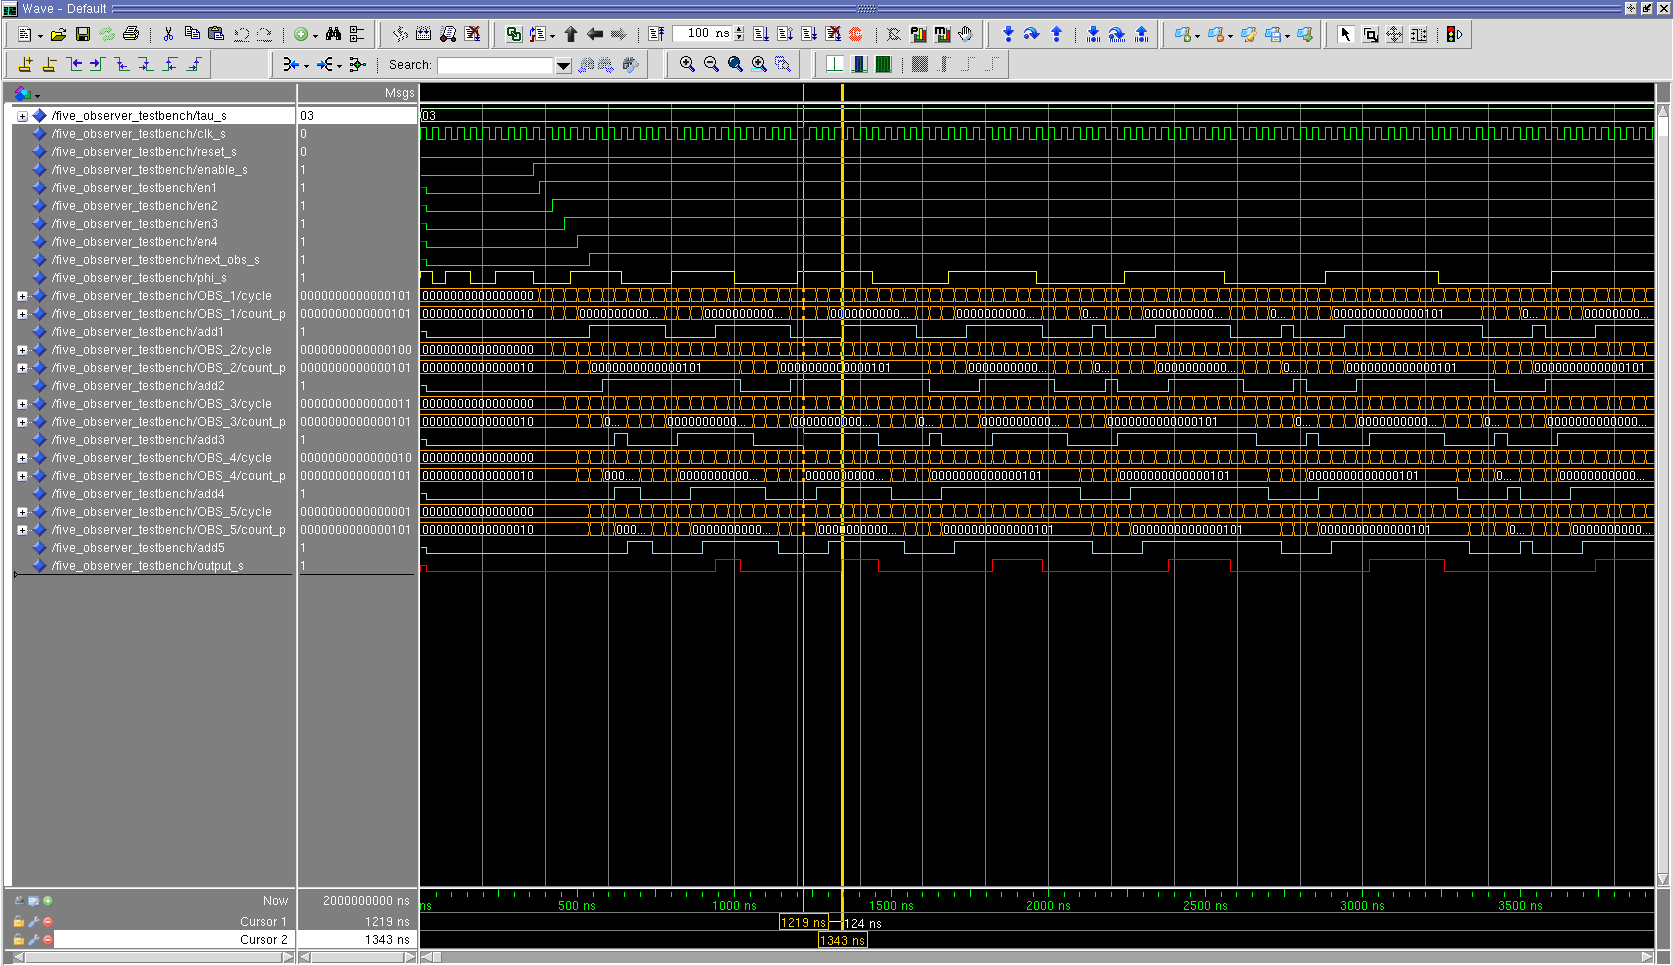
\includegraphics[width=650px,height=300px,angle=-90]{../../pictures/Modelsim/5_Observer_tb_1.png}
%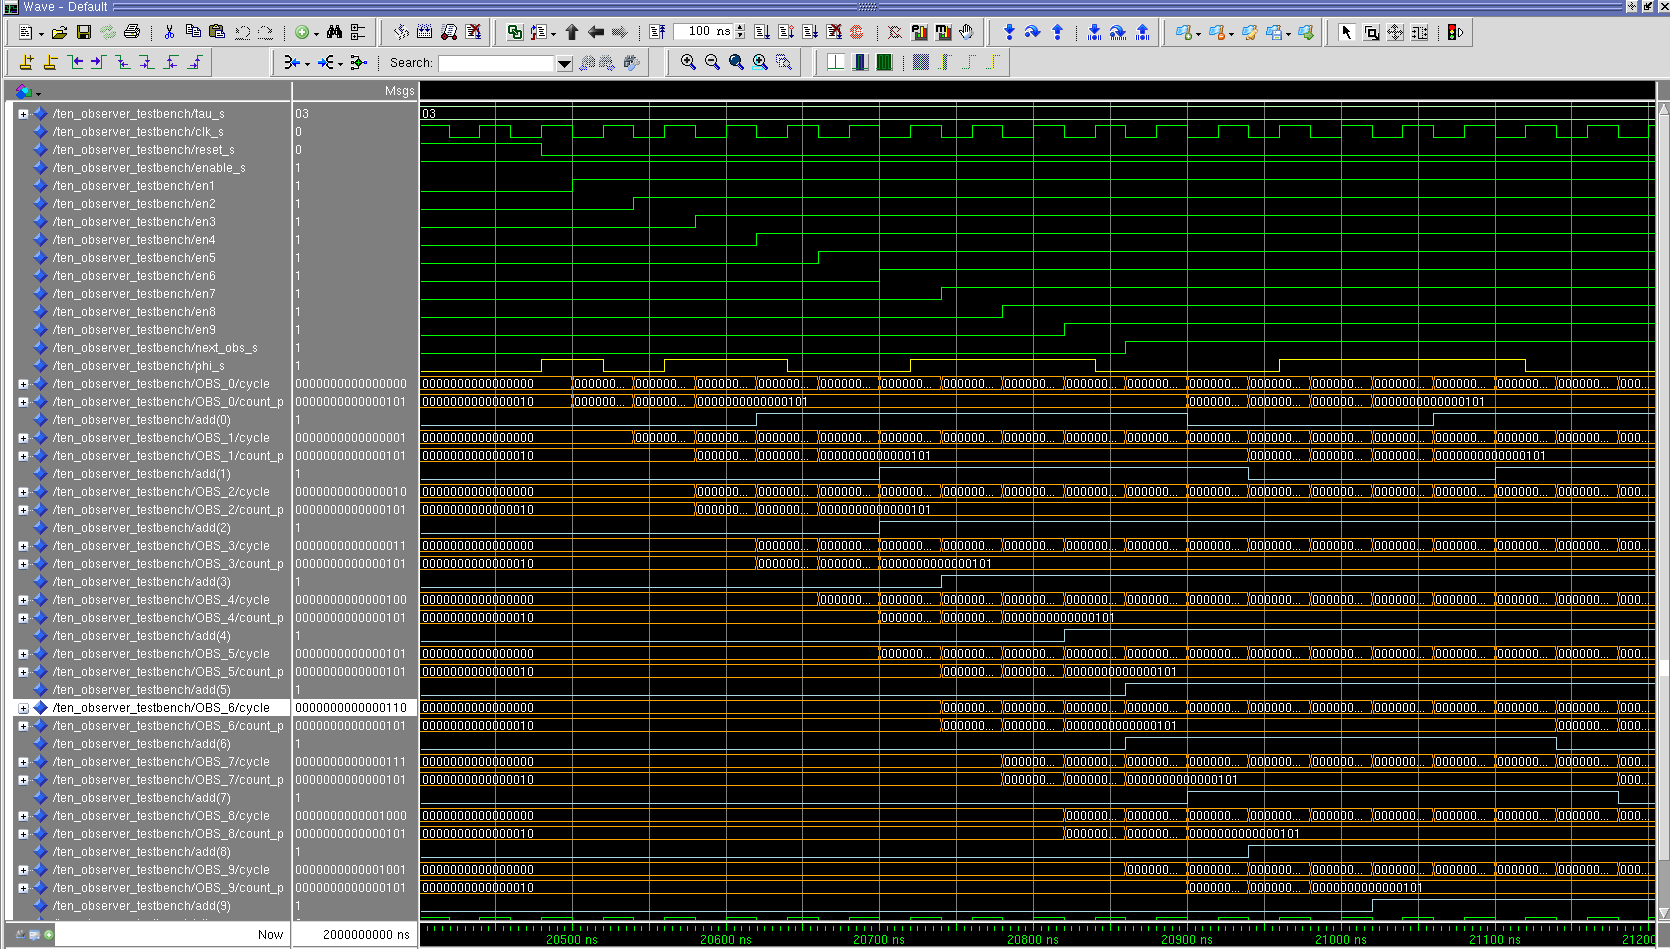
\includegraphics[height]{../../pictures/Modelsim/10_Observer_tb_1.png}
\caption[Modelsim Simulation of 5 Observer]{Illustration of a Simulation with m=5 Observer and Invariance $\tau=3$}
\label{fig:simulation:five}
\end{figure}

\newpage
%C)Simulations
\section{Experiments}
This section treats the experiments done for the Invariance Observer Design. The main part of the experiments were dedicated for testing of the behaviour of the
Invariant Observer Stages. Other experiments were justified by the reason to figure out the maximum performance ot these Observer Stages.
It is decent to presentate only the edge cases of the experiments, which have reasonable arguments, but it is clear that a lot of more test cases where exercised.
Like in the simulation it was important that the behaviour of the Invariant Observer Stages is the same on the FPGA Board and that the timings are correct.
It should be mentioned that no timing simulation where done, because the scope of the bachelor thesis was only to show the behaviour and possibility of this kind of an Invariant Observer. 
The behaviour of the Invariant Observer synthesized on the DE2-115 FPGA board will be shown by pictures of the Logic Analyzer (Agilent 16803A) which were used to monitor
the output pins GPIO(0) to GPIO(34) of the FPGA Board. The pictures shown for up tp 5 Observers shows only GPIO(0) to GPIO(14) from up to down in respective order, for up to 10 Observers shows 
pin GPIO(0) to GPIO(14).For example GPIO(0) is always the reset\_s signal like in Figure~\ref{fig:simulation:five} and so on. 
The names of the signals are the same like in the simulation, so it should be clear wat the signal in the appropriate line means.
\subsection{Testing the Behaviour}
The following examples are implemented with a signalgenerator which was build individually to simulate an increasing invariance.
This is only the case, because we want to see the correct behaviour of the Observer Stages indicated by add0 to addn and final\_output.
The signalgenerator an the observer stages are driven with the same input clock of 50Mhz, only for demonstration.
A indicated $f_{max}$ is meant as the maximum frequency estimation for the whole design according to the Slow 1200mv 85°C model, which was described in subsection Chapter~\ref{chapter:3:section:sub:2}.
But that will be more considered in the next subsection regarding the performance, whereas this section has no significant arguments of the performance, because of the inlcuded signalgenerator.
The names on the left are similar to the names that were already explained in the section before. Now some designate examples:\\
\\
\begin{itemize}
\item The simplest case as the first picture Figure~\ref{fig:logicanalyzer:m1:t1} shows, is one Observer $m = 1$ and $\tau = 1$ .
Like in the simulation explained the vertical lines indicates the start of an Invariance Condition and the start of active signal phi\_s itself.
 \begin{itemize}
 \item $\tau = 1 \;with\; f_{max}=91,41\;Mhz$ (shown in Figure~\ref{fig:logicanalyzer:m1:t1})
 \item $\tau = 10 \;with\; f_{max}=87,61\;Mhz$ 
\end{itemize}

\begin{figure}[]
\centering
%\hspace{-3.0cm}
%\vspace{-5cm}
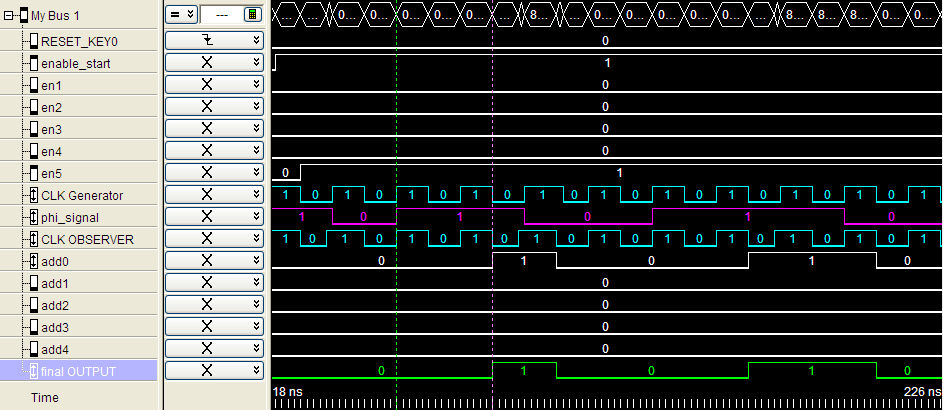
\includegraphics[width=300px,height=150px]{../../pictures/Logicanalyzer/Observer_1_Tau_1.png}
\caption[Logicanalyzer m=1,$\tau=1$]{Illustration from the Logic analyzer which shows the m=1,$\tau = 1$}
\label{fig:logicanalyzer:m1:t1}
\end{figure}



% Figure~\ref{fig:logicanalyzer:m1:t1}
% Figure~\ref{fig:logicanalyzer:m5:t10}
% Figure~\ref{fig:logicanalyzer:m10:t1:1}
% Figure~\ref{fig:logicanalyzer:m10:t1:2}
\item Figure~\ref{fig:logicanalyzer:m5:t10} shows 5 Observer (m=5) with observing Invariance of 10\\


\begin{figure}[]
\centering
%\hspace{-3.0cm}
%\vspace{-5cm}
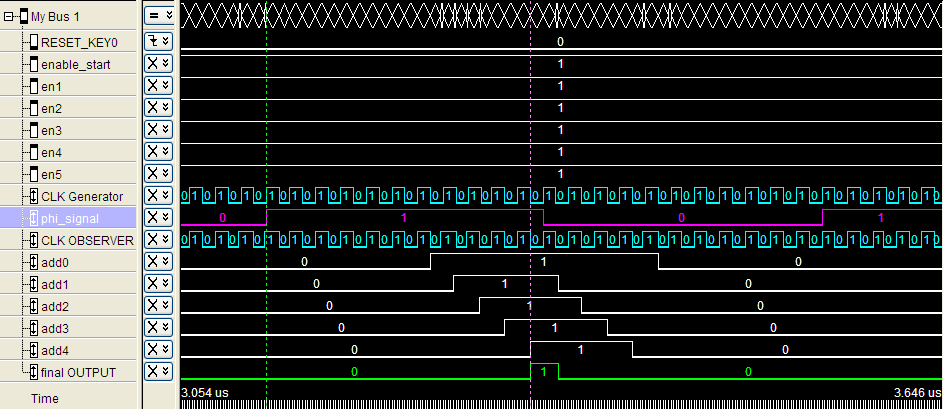
\includegraphics[width=300px,height=150px]{../../pictures/Logicanalyzer/5_Observer_Tau_10.png}
\caption[Logicanalyzer m=5,$\tau=10$]{Illustration from the Logic analyzer which shows the m=1,$\tau = 10$}
\label{fig:logicanalyzer:m5:t10}
\end{figure}

\item Figure~\ref{fig:logicanalyzer:m10:t1:1} shows 10 Observer (m=10) with observing Invariance of 1\\

\begin{figure}[]
\centering
%\hspace{-3.0cm}
%\vspace{-5cm}
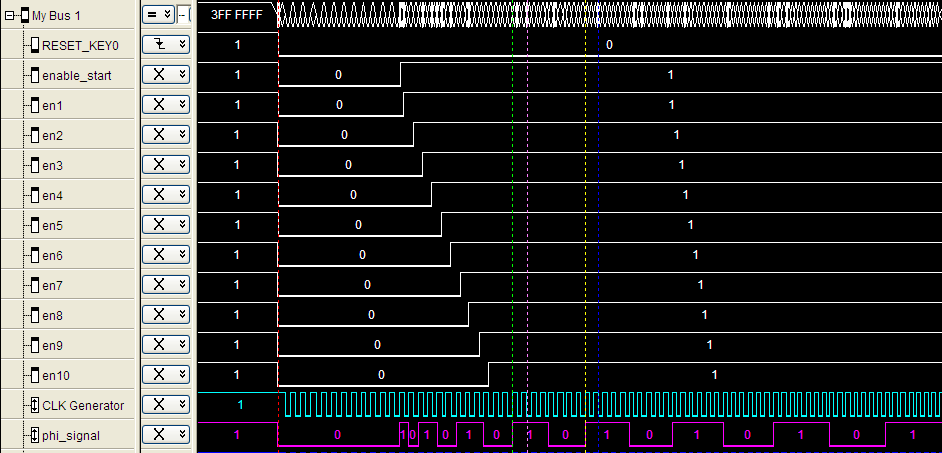
\includegraphics[width=300px,height=150px]{../../pictures/Logicanalyzer/10_Observer_Tau_1_2.png}
\caption[Logicanalyzer m=10,$\tau=1$]{Illustration from the Logic analyzer which shows the m=1,$\tau = 1$}
\label{fig:logicanalyzer:m10:t1:1}
\end{figure}


\begin{figure}[]
\centering
%\hspace{-3.0cm}
%\vspace{-5cm}
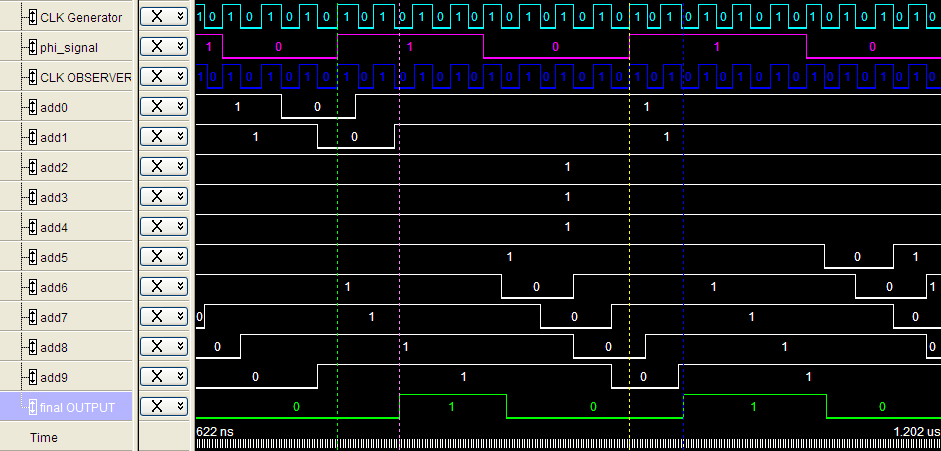
\includegraphics[width=300px,height=150px]{../../pictures/Logicanalyzer/10_Observer_Tau_1_1.png}
\caption[Logicanalyzer m=10,$\tau=1$]{Illustration from the Logic analyzer which shows the m=10,$\tau = 1$}
\label{fig:logicanalyzer:m10:t1:2}
\end{figure}

\end{itemize}

\subsection{Maximum Performance}
